\section{Gaussian process surrogate}

The most popular surrogate model is the Gaussian process, we will now understand model
in more detail. Normally a probabilistic regression model is on the from 
$$y = f_w(x) + \epsilon$$
where weights are trained. $f$ could describe a linear model, $f(x) = w^Tx$ or a polynomial
$f(x) = w\cdot x^2$ etc. the performance of the regression model is very dependend on the 
regression model. The Gaussian process takes a completely different approach, its model $f$ does not
include any parameters. If we collect the data in a vector $\textbf{f} := [f(x_1),\dots,f(x_n)]$
then the GP assign it a multivariate normal distribution, 
$$\textbf{f} \sim \mathcal{N}(\bm{\mu}, \bm{\Sigma})$$

where $\bm{\mu}$ typically is $0$ and the covariance matrix, is depeneded on the input, $x_1, \dots, x_n$, 
 $$\bm{\Sigma} = c(\textbf{x}, \textbf{x}) = \begin{bmatrix}
    c(x_1,x_1) & \dots & c(x_1,x_n)\\
    \vdots& \ddots\\
    c(x_n,x_1) & \dots & c(x_n,x_n)
\end{bmatrix}\hspace{1cm} c(x, y) := Matern(x,y)...$$ 
this means that a realization of the vector $\textbf{f}$ is often close to 0 with a variance of the diagonal $\bm{\Sigma}$,
\todo{NO!! Change}but also with a correlation between the elements in $\textbf{f}$ given by the off-diagonals in $\bm{\Sigma}$. This is a very important
ingredience of a GP, if $c(x_1,x_2) \approx 1$ (assuming that the variances of $\textbf{f}$ is 1, then $\bm{\Sigma}$ is a correlation error)
then realizations of $\textbf{f}$ always lead to similar values of $f(x_1)$ and $f(x_2)$. This encapsulates the idea of a GP: 
similarities (could be distance or other measures) in $x$ should lead to similarities in $f(x)$. Now, in the case of extending it to 
a regression model, we need to bring a unobserved $y_*$ for a arbitrary location $x_*$ into the game. Prior to observing any data, 
we assume that the corresponding $\textbf{f}_*$ is just a new element in the multivariate normal distribution, 
\begin{align}
    p(f(\cdot),\textbf{f}|\textbf{x}) = \mathcal{N}\left(\begin{bmatrix}
        f(\cdot)\\ \textbf{f}
    \end{bmatrix} \middle| \begin{bmatrix}
        0\\ \textbf{0}
    \end{bmatrix}, \begin{bmatrix}
        c(\cdot, \cdot) & c(\cdot,\textbf{x})\\
        c(\textbf{x}, \cdot) & c(\textbf{x}, \textbf{x})
    \end{bmatrix} \right)
\end{align}
yielding many possible outcomes for $\textbf{f}_*$, but with an average $E[\textbf{f}_*] = 0$ and variance of $V[\textbf{f}_*] = 1$.
but note, we treate $\textbf{f}$ as random quantaty, but if get a realization of $\textbf{f}$, then
the distribution of $\textbf{f}_*$ is changed, 
$$p(f(\cdot)|\textbf{x}, \textbf{f}) = \mathcal{N}(f(\cdot)|c(\cdot, \cdot)^{-1}c(\cdot, \textbf{x})\textbf{f}, c(\cdot, \cdot)^{-1})$$

What we want is the predictive posterior distribution, of a new point $p(y_*|x_*, \mathcal{D})$, i.e. by marginalizing 
out the random variabel $f(x_*)$, 
\begin{equation}\label{GP_predictive}
    p(y_*|x_*,\mathcal{D}) = \int \mathcal{N}(y_*|f(x_*), \sigma^2) p(f(x_*)|\mathcal{D})df(x_*)
\end{equation}
where we assume that $\epsilon$ from \ref{..} is a Gaussian with zero mean and variance $\sigma^2$. We will
soon see that the posterior $p(f(x_*)|\mathcal{D})$ is also a normal distribution so using <trick> we end up
with the distribution. 
$$p(y_*|x_*,\mathcal{D}) = \mathcal{N}(y_*|E[f(x_*)], Var(f(x_*))+\sigma^2)$$
So now want to calculate $p(f(x_*)|\mathcal{D})$, 

\begin{equation}\label{posterior_function2}
    p(f(x_*)|\mathcal{D})= \int p(f(x_*)|\textbf{x}, \textbf{f})p(\textbf{f}|\mathcal{D})d\textbf{f}.
\end{equation} 

<image>

Assuming corr

\begin{figure}[h]
    \centering
    \begin{minipage}[b]{0.49\textwidth}
     \includegraphics[trim=1cm 0.7cm 1cm 1cm,clip,width=\textwidth]{Figures/reg_illustrations/GP/Test1_GP_n_10_seed_42.jpg}
    \end{minipage}
    \hfill
    \begin{minipage}[b]{0.49\textwidth}
      \includegraphics[trim=1cm 0.7cm 1cm 1cm,clip,width=\textwidth]{Figures/reg_illustrations/GP/Test2_GP_n_40_seed_42.jpg}
     \end{minipage}
    
     \begin{minipage}[b]{0.49\textwidth}
      \includegraphics[trim=1cm 0.7cm 1cm 1cm,clip,width=\textwidth]{Figures/reg_illustrations/GP/Test3_GP_n_40_seed_42.jpg}
     \end{minipage}
     \hfill
     \begin{minipage}[b]{0.49\textwidth}
       \includegraphics[trim=1cm 0.7cm 1cm 1cm,clip,width=\textwidth]{Figures/reg_illustrations/GP/Test4_GP_n_40_seed_42.jpg}
      \end{minipage}
      \caption{GP tested on all problems.}
\end{figure}

Using a GP as a surrogate model is very popular in Bayesian Optimization, one of the reasons
are its exact inference, and often its assumption is a very good characteristic of the true
function. 

\subsection{Exact predictive distribution}
We now show how the preditive distribution is calculated exact for
Gaussian Processes, i.e. 
\begin{equation}\label{GP_predictive2}
    p(y|x,\mathcal{D}) = \int \mathcal{N}(y|f(x), \sigma^2) p(f(x)|\mathcal{D})df(x)
\end{equation}
we will soon see that $p(f(x)|\mathcal{D}) = \mathcal{N}(f(x)| .., ...)$ and
and thereby that we have a marginal Gaussian distribution for $f(x)$ and a 
conditional Gaussian distribution of $y$ given $f(x)$, giving us the marginalized
distribtuion, $p(y|x,\mathcal{D})$, using formulars \eqref{marginal_distribution}. 

\begin{testexample2}[Trick with normal distributions [from Bishops book?]]
    Given a marginal Gaussian distribution of $x$ and a conditional Gaussian distribution
    of $y$ given $x$ of the form, 
    \begin{align*}
        p(x) &= \mathcal{N}(x|\mu, \Lambda^{-1})\\
        p(y|x) &= \mathcal{N}(x|Ax+b, L^{-1})
    \end{align*}
    then the marginal distribution of $y$ and the conditional distribution of $x$ given $y$
    have the form, 
    \begin{align}
        p(y) &= \mathcal{N}(y|A\mu+b,L^{-1}+A \Lambda^{-1}A^T) \label{marginal_distribution}\\
        p(x|y) &= \mathcal{N}(x|\Gamma \mu+\Gamma [A^TL(y-b)],\Gamma )\\
        \Gamma &:= (\Lambda +A^TLA)^{-1}
    \end{align}
\end{testexample2}

\subsubsection*{Posterior function}
Recall we assume $\textbf{f} = (f(\textbf{x}_1), \dots, f(\textbf{x}_n))$ is the parameters in 
our model, therefore we call $p(\textbf{f}|\mathcal{D})$ the posterior distribution. However, 
what is of real interest is the function values on unobserved locations, thereby we 
extend $\textbf{f}$ to be a function, i.e. an infinitely dimentional vector. We call this 
quantaty \textit{the posterior function} 
\begin{equation}\label{posterior_function}
    p(f(\cdot)|\mathcal{D})= \int p(f(\cdot)|\textbf{x}, \textbf{f})p(\textbf{f}|\mathcal{D})d\textbf{f}.
\end{equation}
% The connection between the two posteriors is given here:
% $$p(f(\cdot)|\mathcal{D}) = \int p(f(\cdot)|\textbf{x}, \textbf{f})p(\textbf{f}|\mathcal{D})d\textbf{f}$$
Prior we assume that the function takes values accoring to
$$p(\textbf{f}|\textbf{x}) = \mathcal{N}(\textbf{f}|\textbf{0}, c(\textbf{x}, \textbf{x}))$$ where
the covariance is defined at kernel evaluation for each pair of $\textbf{x}$, where $c(\cdot,
\cdot)$ is a covariance function, chosen to be the Matérn covariance function,

  $$c(\textbf{x}, \textbf{x}) = \begin{bmatrix}
    c(x_1,x_1) & \dots & c(x_1,x_n)\\
    \vdots& \ddots\\
    c(x_n,x_1) & \dots & c(x_n,x_n)
\end{bmatrix}\hspace{1cm} c(x, y) := Matern(x,y)...$$ 

\begin{figure}[h]
    \centering
    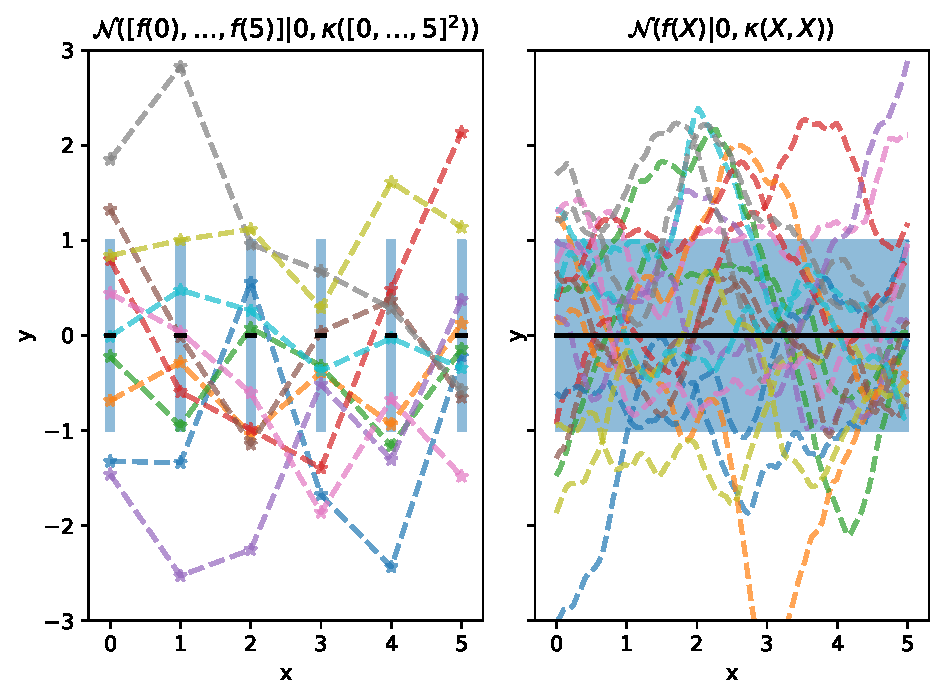
\includegraphics[width = \textwidth]{Pictures/GP_samples_mattern.pdf}
    \caption{Realisations> Illustartaion of GP is just samples from a multivariate normal distribution. In the
    limit the we have a infinite-variate normal distribution, which we call a GP.}
\end{figure}

Appendix <...> tries to give the intuition why this makes sense. 

We now calculate the first term in the integral \eqref{posterior_function}, 
$p(f(\cdot)|\textbf{x}, \textbf{f})$ using that we have the joint prior 
distribution, 
\begin{align}
    p(f(\cdot),\textbf{f}|\textbf{x}) = \mathcal{N}\left(\begin{bmatrix}
        f(\cdot)\\ \textbf{f}
    \end{bmatrix} \middle| \begin{bmatrix}
        0\\ \textbf{0}
    \end{bmatrix}, \begin{bmatrix}
        c(\cdot, \cdot) & c(\cdot,\textbf{x})\\
        c(\textbf{x}, \cdot) & c(\textbf{x}, \textbf{x})
    \end{bmatrix} \right)
\end{align}

And the conditonal of a joint Gaussian is given using <ref> 
$$p(f(\cdot)|\textbf{x}, \textbf{f}) = \mathcal{N}(f(\cdot)|c(\cdot, \cdot)^{-1}c(\cdot, \textbf{x})\textbf{f}, c(\cdot, \cdot)^{-1})$$

Next we calculate the last term in the integral \eqref{posterior_function}, 
$p(\textbf{f}|\mathcal{D})$, i.e. the posterior distribution. Assuming iid data, 
i.e. $p(y_1,\dots, y_n|x_1,\dots, x_n, \textbf{f}) = \prod_{i=1}^n p(y_i|x_i,\textbf{f}_i)$
and that the likelihood is Gaussian with mean $\textbf{f}$ and variance $\sigma^2 I_n$. 

\begin{align*}
    p(\textbf{f}|\mathcal{D}) &\propto p(\textbf{f}|x)\prod_{i=1}^n p(y_i|x_i,\textbf{f}_i)\\
    &= \mathcal{N}(\textbf{f}|\textbf{0},c(\textbf{x}, \textbf{x})) \prod_{i=1}^n \mathcal{N}(y|\textbf{f}_i,\sigma^2)\\
    &= \mathcal{N}(\textbf{f}|\textbf{0}, c(\textbf{x}, \textbf{x})) \mathcal{N}(\textbf{y}|\textbf{f},\sigma^2 I_n)
\end{align*}
now from <ref> we have that the posterior is the following Gaussian: 
\begin{equation*}
    p(\textbf{f}|\mathcal{D}) = \mathcal{N}(\textbf{f}|M^{-1} \sigma^{-2}\textbf{y}, M^{-1}) \hspace{0.5cm}M := c(\textbf{x}, \textbf{x})^{-1}+\sigma^{-2} I_n
\end{equation*}
Now we found that both term in the integral \eqref{posterior_function}, and they
are related such that it is possible to use \eqref{marginal_distribution} for arriving 
at (we define $A :=  c(\cdot, \cdot)^{-1} c(\cdot, \textbf{x})$), 
$$p(f(\cdot)|\mathcal{D}) = \mathcal{N}(f(\cdot)|AM^{-1}\sigma^{-2}\textbf{y}, c(\cdot, \cdot)^{-1}+
AM^{-1}A^T)$$

Finally we found that both terms in the integral \eqref{GP_predictive} also is related
in a simlar way, and we use \eqref{marginal_distribution}, again to arrive at the predictive
distribtuion, 
$$p(y_*|x_*,\mathcal{D}) = \mathcal{N}(y_*|AM^{-1}\sigma^{-2}\textbf{y}, c(x_*, x_*)^{-1}+
AM^{-1}A^T+\sigma^2)$$

\subsubsection*{Learning - Emperical bayes inference}

Another inference which is done is then optimizing the hyper parameters using emperical bayes i.e.
the variance and length scale for the kernel. Here we optimize the marginalized likelihood function
$$p(y_1, \dots, y_n|x_1, \dots, x_n, \theta) = -\frac{1}{2}[(y-\mu)^T (\Sigma+N)^{-1}(y-\mu)+ \log |\Sigma+N|+n \log 2\pi]$$
<and how to get to there?>

\todo{Model assessment becomes trivial in light of the model posterior if we
simply establish preferences over models according to their posterior
probability. When using the uniform model prior (4.6)
 the model posterior is proportional to the marginal likelihood alone,
which can be then used directly for model assessment. ??! Youtube - good video! Go through that!}

